\section{Hyperbolic geometry}

\subsection{Normal polygons and fundamental regions}

%Vonroi diagram

\begin{figure}
\centering
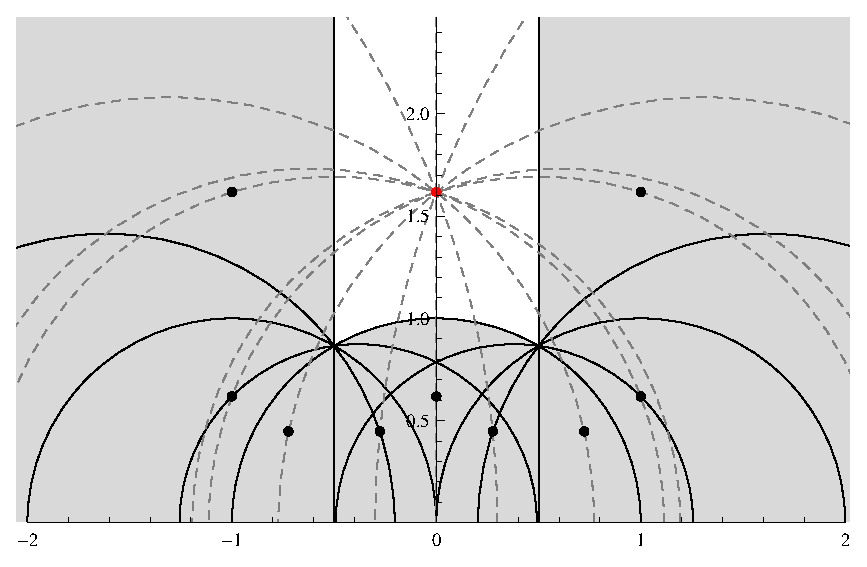
\includegraphics[width=\textwidth]{figures/normpoly-fundom-1}
\caption[The fundamental domain $\FunDom$ as normal polygon]{The fundamental domain $\FunDom$ can alternatively obtained by constructing the normal polygon with respect to any point $z$ on the imaginary axis with $\Im{z} > 1$. Above the point $z = \phi \ii$ (red) has been chosen, where $\phi = \frac{\sqrt{5}+1}{2}$ denotes the golden ratio.}
\label{fig_NormalPolyFunDom}
\end{figure}

\begin{figure}
\centering
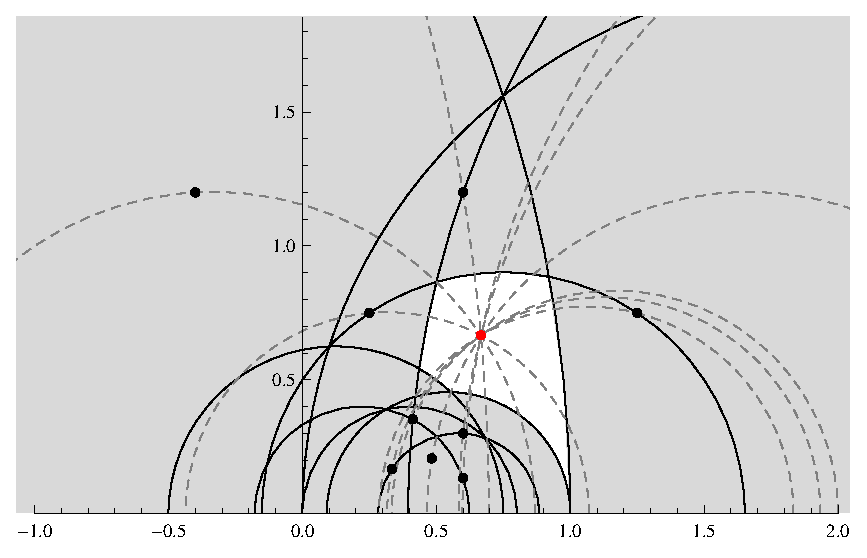
\includegraphics[width=\textwidth]{figures/normpoly-fundom-2}
\caption[An alternative fundamental domain for $\PSL{\Z}$]{An alternative fundamental domain for the action of $\PSL{\Z}$ on $\EU$. It is obtained by constructing the normal polygon for the point $\frac{2}{3}(1+\ii)$.}
\label{fig_AltNormalPolyFunDom}
\end{figure}
